\documentclass{article}

\usepackage{arxiv}

\usepackage[utf8]{inputenc}   % entrada UTF-8 (acentos)
\usepackage[T1]{fontenc}      % fuentes de 8 bits
\usepackage[spanish,es-tabla,es-noshorthands,es-nodecimaldot]{babel}
\usepackage[table]{xcolor}    % colores
\usepackage{hyperref}         % hipervínculos
\usepackage{xurl}             % URLs (permite cortar en cualquier carácter)
\usepackage{booktabs}         % tablas profesionales
\usepackage{amsfonts}         % símbolos matemáticos
\usepackage{amsmath}          % ecuaciones
\usepackage{nicefrac}         % fracciones compactas
\usepackage{microtype}        % microtipografía
\usepackage{graphicx}         % figuras
\usepackage{array}            % columnas con formato
\usepackage{longtable}        % tablas de más de una página
\usepackage{placeins}         % \FloatBarrier
\usepackage[numbers,sort&compress]{natbib} % citas numéricas
\usepackage{caption}          % leyendas
\captionsetup{font=small, labelfont=bf}
\hypersetup{colorlinks=true, linkcolor=blue!50!black, citecolor=blue!50!black,
            urlcolor=blue!50!black}
\graphicspath{{../figures/}}

% Etiquetas del template arxiv.sty traducidas al español (el estilo no se modifica)
\def\keywordname{{\bfseries \emph{Palabras clave}}}
\renewenvironment{abstract}
  {\centerline{\large \bfseries \scshape Resumen}\begin{quote}}
  {\end{quote}}
\rhead{\scshape Trabajo práctico - UCA - \today}

% Cifras generadas automáticamente por el código R (results/numeros.tex):
% cada número del informe coincide exactamente con lo que produce el código.
\newcommand{\nEncBal}{14}
\newcommand{\nSim}{20.000}
\newcommand{\muBal}{49,9}
\newcommand{\muBalK}{50,1}
\newcommand{\muBalMayo}{60,1}
\newcommand{\dispBal}{2,9}
\newcommand{\rmseMargen}{8,5}
\newcommand{\sigmaEnc}{4,3}
\newcommand{\sigmaDeriva}{5,0}
\newcommand{\sigmaTotal}{6,6}
\newcommand{\pvLLA}{45,8}
\newcommand{\pvSinproLLA}{40,0}
\newcommand{\pvPJ}{35,7}
\newcommand{\pvSinproPJ}{35,7}
\newcommand{\pvFIT}{7,7}
\newcommand{\pvSinproFIT}{7,7}
\newcommand{\pvPU}{5,5}
\newcommand{\pvSinproPU}{5,5}
\newcommand{\pvOTROS}{5,3}
\newcommand{\pvSinproOTROS}{11,1}
\newcommand{\muDelta}{11,4}
\newcommand{\sdDelta}{9,9}
\newcommand{\cambioNac}{-0,1}
\newcommand{\pMileiHoy}{68,1}
\newcommand{\pKiciHoy}{31,9}
\newcommand{\pBalHoy}{40,3}
\newcommand{\pMileiPVHoy}{57,6}
\newcommand{\pKiciPVHoy}{2,1}
\newcommand{\pMileiCondHoy}{26,2}
\newcommand{\pMileiA}{66,2}
\newcommand{\pKiciA}{33,8}
\newcommand{\pBalA}{35,3}
\newcommand{\pMileiPVA}{55,5}
\newcommand{\pKiciPVA}{9,2}
\newcommand{\pMileiCondA}{30,4}
\newcommand{\pMileiB}{55,4}
\newcommand{\pKiciB}{44,6}
\newcommand{\pBalB}{52,2}
\newcommand{\pMileiPVB}{33,8}
\newcommand{\pKiciPVB}{14,0}
\newcommand{\pMileiCondB}{41,4}
\newcommand{\pMileiC}{50,2}
\newcommand{\pKiciC}{49,8}
\newcommand{\pBalC}{47,6}
\newcommand{\pMileiPVC}{27,8}
\newcommand{\pKiciPVC}{24,6}
\newcommand{\pMileiCondC}{47,2}
\newcommand{\pMileiFinal}{60,8}
\newcommand{\pKiciFinal}{39,2}
\newcommand{\pBalFinal}{43,8}
\newcommand{\pMileiPVFinal}{44,6}
\newcommand{\pKiciPVFinal}{11,6}
\newcommand{\pMileiCondFinal}{35,9}
\newcommand{\votoLLAFinal}{42,9}
\newcommand{\votoPJFinal}{35,6}
\newcommand{\votoLLAFinalLo}{31,0}
\newcommand{\votoLLAFinalHi}{55,4}
\newcommand{\votoPJFinalLo}{24,0}
\newcommand{\votoPJFinalHi}{47,0}
\newcommand{\balMedTodas}{49,9}
\newcommand{\balMedCond}{48,2}
\newcommand{\balMedCondK}{51,8}
\newcommand{\pKiciBalFinal}{27,6}
\newcommand{\pMileiBalFinal}{16,2}
\newcommand{\pvCandLLA}{40,8}
\newcommand{\pvCandPJ}{40,1}
\newcommand{\pvCandFIT}{11,0}
\newcommand{\pMileiDerivaCero}{68,9}
\newcommand{\pMileiDerivaSiete}{65,2}
\newcommand{\nEfecto}{7}
\newcommand{\muDeltaGob}{20,5}
\newcommand{\muDeltaLeg}{7,8}
\newcommand{\gobLLAMed}{10}
\newcommand{\gobLLALo}{6}
\newcommand{\gobLLAHi}{14}
\newcommand{\gobLLAMedia}{9,9}
\newcommand{\gobPJMed}{7}
\newcommand{\gobPJLo}{4}
\newcommand{\gobPJHi}{10}
\newcommand{\gobPJMedia}{7,0}
\newcommand{\gobPROVMed}{5}
\newcommand{\gobPROVLo}{2}
\newcommand{\gobPROVHi}{8}
\newcommand{\gobPROVMedia}{4,9}
\newcommand{\gobOtrosMed}{0}
\newcommand{\gobOtrosLo}{0}
\newcommand{\gobOtrosHi}{1}
\newcommand{\gobOtrosMedia}{0,2}
\newcommand{\cambiosEsperados}{4,5}
\newcommand{\nOfiFavorito}{22}
\newcommand{\pTodosRetienen}{1,5}
\newcommand{\medOfiRetienen}{17}
\newcommand{\pSantaFeBase}{45,3}
\newcommand{\pSantaFeAlt}{99,7}
\newcommand{\pCabaBase}{97,1}
\newcommand{\pCabaAlt}{42,4}
\newcommand{\pPBA}{81,2}
\newcommand{\medPBAofi}{50,8}
\newcommand{\medPBAseg}{33,9}
\newcommand{\pJujuy}{46,9}
\newcommand{\pSantaCruz}{37,3}
\newcommand{\pChubut}{77,7}
\newcommand{\pRioNegro}{64,3}
\newcommand{\pCordoba}{87,0}
\newcommand{\pSantaFe}{72,5}
\newcommand{\pCaba}{69,7}
\newcommand{\nEncProv}{3}
\newcommand{\nFilasDatos}{123}
\newcommand{\fechaCorte}{19/11/2026}

% Las filas de las tablas se insertan con el \input primitivo de TeX: el
% \input de LaTeX rompe las reglas de booktabs (\bottomrule) dentro de un tabular.
\makeatletter
\newcommand{\tablainput}[1]{\@@input #1 }
\makeatother
\newcommand{\pp}{\,pp}
\newcolumntype{L}[1]{>{\raggedright\arraybackslash}p{#1}} % columna alineada a la izquierda

\title{¿Quién gobierna desde 2027?\\[0.3em]
\large Simulación Monte Carlo de las elecciones presidenciales y de
gobernadores de Argentina con encuestas reales, resultados 2023--2025 y el
error histórico de las encuestas}

\author{
  Matías Costabile \\
  Licenciatura en Ciencia de Datos\\
  Pontificia Universidad Católica Argentina (UCA)\\
  Buenos Aires, Argentina \\
  \texttt{matycostabile2008@gmail.com} \\
}

\begin{document}
\maketitle

\begin{abstract}
Faltan once meses para las elecciones de octubre de 2027 y las encuestas
publicadas no coinciden entre sí: algunas muestran a Javier Milei arriba y otras
a Axel Kicillof. Este trabajo junta todos esos datos y simula la elección
\nSim{} veces para responder con probabilidades, no con certezas, quién sería
presidente y quién ganaría cada una de las 22 gobernaciones que se eligen en 2027
(21 provincias y la Ciudad Autónoma de Buenos Aires; Corrientes y Santiago del
Estero ya eligieron en 2025). Se usan \nEncBal{} encuestas de balotaje y un
promedio de once encuestadoras, encuestas de primera vuelta, los resultados
reales de Diputados 2025 en cada distrito, siete elecciones provinciales de 2025
para medir la ventaja del oficialismo local y cuatro elecciones de 2023--2025
para medir cuánto se equivocan las encuestas en Argentina (\rmseMargen\pp{} de
error cuadrático medio en el margen). Cada dato tiene su fuente. Las encuestas
de balotaje dan un empate (\muBal\% para Milei sobre los votos válidos), pero las
reglas de la primera vuelta y la ventaja que hoy muestra La Libertad Avanza (LLA)
cuando se mide por espacios hacen que el \textbf{resultado final} de la
simulación sea: \textbf{Milei reelecto con una probabilidad de \pMileiFinal\%} y
Kicillof presidente con \pKiciFinal\%. Hay balotaje en el \pBalFinal\% de las
simulaciones y, cuando lo hay, Kicillof lo gana más veces que Milei (Milei gana
sólo el \pMileiCondFinal\% de los balotajes). El resultado depende mucho de si el
PRO va aliado con LLA (\pMileiA\% contra \pMileiB\%) y de qué encuestas se miran
(con las que preguntan por candidatos queda \pMileiC\% a \pKiciC\%). En las
provincias, el oficialismo es favorito en los \nOfiFavorito{} distritos, pero se
esperan en promedio \cambiosEsperados{} cambios de signo; los más disputados son
Santa Cruz, Jujuy y Río Negro. Es una simulación, no una predicción.
\end{abstract}

\keywords{Elecciones \and Argentina \and Encuestas \and Simulación Monte Carlo
\and Agregación de encuestas \and Error de encuestas \and Gobernadores}

% =====================================================================
\section{Objetivo}

El objetivo de este trabajo es \textbf{construir una simulación reproducible,
basada sólo en datos públicos con fuente, de las elecciones argentinas de 2027}:
la presidencial (primera vuelta y, si corresponde, balotaje) y las de los 21
gobernadores y el jefe de Gobierno de la Ciudad Autónoma de Buenos Aires que se
eligen ese año. En concreto se busca:

\begin{enumerate}
  \item Reunir en datasets abiertos todas las encuestas nacionales y provinciales
        publicadas en 2026 que pudieron encontrarse, los resultados oficiales
        de 2023 y 2025 y el estado de cada candidatura, con la fuente de cada fila.
  \item Combinar las encuestas en un promedio ponderado por tamaño de muestra y
        antigüedad.
  \item Medir con datos argentinos cuánto se equivocan las encuestas y cuánta
        ventaja tiene el oficialismo provincial, en lugar de suponerlo.
  \item Simular la elección miles de veces aplicando las reglas de la
        Constitución (artículos 94 a 98) y dar un \textbf{resultado final} con
        su probabilidad: quién gana la presidencia, si hay balotaje y quién lo
        gana, y quién gana cada gobernación.
  \item Mostrar de qué supuestos depende ese resultado y cuánto cambia si los
        supuestos cambian.
\end{enumerate}

El trabajo no toma partido: los candidatos se eligen por ser los que miden las
encuestas, los colores de los gráficos no son los de ningún partido y todos los
espacios se tratan con el mismo método.

% =====================================================================
\section{Introducción}

\subsection{Contexto}

En octubre de 2027 Argentina elige presidente, renueva parte del Congreso y la
mayoría de las provincias elige gobernador (algunas en la misma fecha y otras en
fechas propias). El presidente Javier Milei (La Libertad Avanza) puede buscar un
segundo mandato consecutivo. En el peronismo no hay candidato definido; el
nombre más medido por las encuestadoras es el del gobernador bonaerense Axel
Kicillof (Fuerza Patria). Las encuestas también miden a Myriam Bregman (Frente
de Izquierda) y a Juan Schiaretti (Provincias Unidas). Este trabajo usa esos
cuatro nombres porque son los que aparecen en las encuestas publicadas; no
implica que vayan a ser candidatos.

A un año de la elección, las encuestas dicen cosas distintas. El promedio de
once encuestadoras publicado por Clarín da a Milei 42,2\% contra 38,9\% de
Kicillof en un balotaje \cite{clarin2026}; otras encuestas recientes, como
Tendencias (36,9\% contra 47,4\%), dan lo contrario. A eso se suma que las
encuestas argentinas fallaron por mucho en las últimas elecciones: en la
provincia de Buenos Aires en 2025 ninguna encuestadora acertó
\cite{chequeadopba2025} y en la Ciudad de Buenos Aires sólo 3 de 11 dieron
ganador al candidato que ganó \cite{chequeadocaba2025}. Mirar una sola encuesta,
entonces, sirve de poco. Lo que sí puede hacerse es combinarlas todas, medir su
error histórico y traducir esa incertidumbre en probabilidades.

\subsection{Resumen del trabajo}

Se armaron ocho datasets con \nFilasDatos{} filas de datos reales, cada una con su fuente
(sección~\ref{sec:datos}). Las encuestas de balotaje se combinan en un promedio
ponderado; las de primera vuelta se convierten a votos afirmativos, que es lo que
cuenta la Constitución. La incertidumbre se calibra con el error real de las
encuestas en cuatro elecciones de 2023--2025 y con un supuesto explícito sobre
cuánto puede cambiar la opinión en once meses. Con eso se simulan \nSim{}
elecciones presidenciales en cuatro escenarios. Para las provincias se parte del
resultado real de Diputados 2025 en cada distrito, se le aplica el cambio
nacional que muestran las encuestas y una ventaja del oficialismo local medida
con siete elecciones provinciales de 2025, y se simulan las 22 gobernaciones.

\subsection{Estado del arte}

\textbf{Las encuestas a un año de la elección.} \citet{gelman1993} mostraron
que las encuestas de campaña oscilan mucho aunque el resultado final sea
bastante predecible, porque los votantes recién se definen cerca de la elección.
\citet{erikson2012} estudiaron cómo las preferencias se van fijando a lo largo
del año electoral y muestran que las encuestas lejanas a la elección predicen
bastante peor que las del final. \citet{jennings2018}, con más de 30.000
encuestas de 351 elecciones en 45 países, encuentran que el error de las
encuestas es estable en el tiempo (no hay una ``crisis'' reciente), pero que
baja a medida que se acerca la elección y que varía según el sistema político;
\citet{jennings2020} discuten específicamente cuánto se puede pronosticar con
mucha anticipación. Esto justifica sumar al error de las encuestas una
incertidumbre adicional por la distancia a la elección (sección~\ref{sec:incert}).

\textbf{El error real es mayor que el margen de error informado.}
\citet{shirani2018} analizaron miles de encuestas estatales en EE.\,UU. y
encontraron que el error total es aproximadamente el doble del margen de error
que publican las encuestadoras, porque además del muestreo hay sesgos de
cobertura, de no respuesta y de modelo de votante probable. Por eso aquí el
error se calibra con resultados reales y no con el margen de error teórico.

\textbf{Modelos de pronóstico por agregación.} \citet{linzer2013} propuso un
modelo bayesiano dinámico que combina encuestas estado por estado con un
pronóstico estructural y comparte información entre estados.
\citet{heidemanns2020} actualizaron ese enfoque para el modelo de \emph{The
Economist} en 2020 y destacan que los errores de los distintos estados están
correlacionados: si las encuestas fallan en uno, suelen fallar en el mismo
sentido en los demás. El modelo provincial de este trabajo incorpora esa idea
con un shock nacional común a todos los distritos. La herramienta de cálculo es
el método de Monte Carlo \cite{metropolis1949}: simular muchas veces un sistema
con componentes aleatorios y contar cuántas veces ocurre cada resultado.

\textbf{La ventaja del oficialismo.} \citet{gelman1990} propusieron cómo medir
sin sesgo la ventaja electoral de quien ya ocupa el cargo. En Argentina,
\citet{gervasoni2010} muestra que los gobernadores de provincias que dependen
mucho de transferencias federales concentran recursos que les dan ventajas
electorales sobre la oposición. Las elecciones provinciales de 2025, en las que
casi todos los oficialismos ganaron, son consistentes con esa idea; aquí esa
ventaja se mide con datos de 2025 (sección~\ref{sec:prov}).

\textbf{Promedios de encuestas para 2027.} En la prensa argentina hay al menos
dos promedios recientes: el de Clarín, con once encuestadoras
\cite{clarin2026}, y uno difundido por La Capital de Mar del Plata con una
docena de encuestas, que da a Milei 33,1\% contra 25,7\% de Kicillof en primera
vuelta \cite{lacapital2026}. Ese segundo trabajo advierte que la mayoría de los
sondeos mide al peronismo kirchnerista separado del no kirchnerista, lo que baja
el número de Fuerza Patria, y mide al PRO por separado de LLA. Ninguno de los dos
traduce los números en probabilidades ni incorpora el error histórico.

\subsection{Aportes de este trabajo}

\begin{itemize}
  \item Un conjunto de datos abierto, con la fuente de cada fila, sobre la
        elección argentina de 2027 (encuestas, candidaturas y resultados previos).
  \item Una calibración del error de las encuestas y de la ventaja del
        oficialismo provincial con datos argentinos de 2023--2025.
  \item Una simulación que aplica las reglas reales de la primera vuelta
        (45\%, o 40\% con 10 puntos de diferencia) y que tiene en cuenta que el
        error de la primera vuelta y el del balotaje están relacionados.
  \item Un resultado final con probabilidades para la presidencia y las 22
        gobernaciones, y un análisis de sensibilidad a los supuestos.
\end{itemize}

% =====================================================================
\section{Datos}
\label{sec:datos}

Todos los datos son públicos y fueron relevados hasta el \fechaCorte. Cada CSV
tiene una columna \texttt{fuente} con el enlace al artículo o tabla de donde sale
cada dato (tabla~\ref{tab:datasets}). No se inventó ningún número: cuando un dato
no existe (por ejemplo, un candidato no definido) figura como ``a definir''.

\begin{table}[htbp]
\centering
\caption{Datasets del trabajo (carpeta \texttt{data/}).}
\label{tab:datasets}
\small
\begin{tabular}{L{4.9cm}L{7.8cm}r}
\toprule
Archivo & Contenido & Filas \\
\midrule
\texttt{encuestas\_balotaje.csv} & Encuestas nacionales de balotaje Milei vs.
Kicillof publicadas en 2026 (incluye el promedio de 11 encuestadoras de Clarín) & 15 \\
\texttt{encuestas\_primera\_vuelta.csv} & Intención de voto en primera vuelta
por espacio y por candidato & 3 \\
\texttt{errores\_historicos.csv} & Margen que daban las encuestas y margen real
en 2023 y 2025 & 4 \\
\texttt{provincias\_2025.csv} & Resultado de Diputados nacionales 2025: tres
fuerzas más votadas en cada distrito \cite{c5n2025} & 66 \\
\texttt{distritos\_2027.csv} & Gobernador actual, si puede ser reelecto,
candidatos mencionados y estado de la alianza con LLA en cada distrito & 22 \\
\texttt{efecto\_oficialismo.csv} & Siete elecciones provinciales de 2025
comparadas con la legislativa nacional & 7 \\
\texttt{encuestas\_provinciales.csv} & Encuestas de gobernador (Córdoba, Santa
Fe, Buenos Aires) & 3 \\
\texttt{caba\_mayo\_2025.csv} & Elección legislativa porteña de mayo de 2025
(LLA, peronismo y PRO por separado) & 3 \\
\texttt{fuente\_resultados\_2025.txt} & Fuentes y totales nacionales 2025 & -- \\
\bottomrule
\end{tabular}
\end{table}

La tabla~\ref{tab:encuestas} lista las encuestas de balotaje con su peso en el
promedio (sección~\ref{sec:promedio}) y la tabla~\ref{tab:pv} las de primera
vuelta. Hay dos tipos de encuesta de primera vuelta: las que preguntan por
\emph{espacios} (el promedio de Clarín, donde el PRO figura aparte y ``otros''
incluye blanco y nulo) y las que preguntan por \emph{candidatos} (Tendencias y
Hugo Haime, que no miden al PRO por separado).

\begin{table}[htbp]
\centering
\caption{Encuestas de balotaje Milei vs. Kicillof usadas (\% de intención de
voto). ``\% válidos'' es la proporción de Milei sobre los votos de ambos; ``Peso''
es su participación en el promedio. s/d: sin dato de muestra (se asume 1.000).}
\label{tab:encuestas}
\footnotesize
\begin{tabular}{lcrrrrrc}
\toprule
Encuestadora & Fecha & $n$ & Milei & Kicillof & \% válidos & Peso (\%) & Fuente \\
\midrule
\tablainput{../results/tabla_encuestas_balotaje.tex}
\bottomrule
\end{tabular}
\end{table}

\begin{table}[htbp]
\centering
\caption{Encuestas de primera vuelta (\% de intención de voto, con blancos e
indecisos). En las encuestas por candidato el PRO no se mide por separado.}
\label{tab:pv}
\footnotesize
\begin{tabular}{lcrrrrrrrc}
\toprule
Fuente & Fecha & LLA & PRO & Peron. & FIT-U & PU & Otros & Bl./NS & Link \\
\midrule
\tablainput{../results/tabla_encuestas_pv.tex}
\bottomrule
\end{tabular}
\end{table}

Para las provincias se usan los resultados de Diputados nacionales del
26/10/2025 en cada distrito (escrutinio provisorio, 98,85\% de mesas)
\cite{c5n2025}. Allí LLA compitió aliada con el oficialismo, o con su apoyo, en cinco distritos
(Chaco, Entre Ríos, Mendoza, San Luis y la Ciudad de Buenos Aires), lo que se
respeta en el modelo. La situación de cada gobernación (si el gobernador puede
ser reelecto, quiénes son los candidatos mencionados y si hay acuerdo con LLA)
está en la tabla~\ref{tab:candidatos} del anexo, con su fuente.

\FloatBarrier
% =====================================================================
\section{Metodología}

\subsection{Promedio ponderado de encuestas}
\label{sec:promedio}

Para el balotaje se usa la proporción de Milei sobre los votos de ambos
candidatos, que es lo que define un balotaje (los votos en blanco no cuentan):
\begin{equation}
  p_i = \frac{\text{Milei}_i}{\text{Milei}_i + \text{Kicillof}_i}.
\end{equation}
Cada encuesta $i$ recibe un peso que crece con el tamaño de la muestra y cae con
la antigüedad:
\begin{equation}
  w_i = \sqrt{\min(n_i,\,3000)}\;\cdot\;0{,}5^{\,d_i/45},
  \qquad \hat{\mu} = \frac{\sum_i w_i\,p_i}{\sum_i w_i},
\end{equation}
donde $n_i$ es el tamaño de la muestra (1.000 si no se informa), $d_i$ los días
transcurridos hasta el \fechaCorte{} y 45 días es la \emph{vida media}: una
encuesta de hace 45 días vale la mitad que una de hoy. La raíz cuadrada refleja
que el error de muestreo baja con $\sqrt{n}$, y el tope de 3.000 evita que una
encuesta online gigante domine el promedio. El promedio de Clarín resume once
encuestadoras, de las cuales tres (CELAG, Proyección y RDT) ya están en la base,
así que pesa como ocho encuestas.

\subsection{Votos afirmativos y reglas constitucionales}

La Constitución define la primera vuelta sobre los \emph{votos afirmativos
válidamente emitidos} \cite{constitucion}, es decir, sin blancos ni nulos. Por
eso cada encuesta de primera vuelta se reparte proporcionalmente entre las
fuerzas, sin blancos ni indecisos:
\begin{equation}
  v_{ik} = 100\,\frac{x_{ik}}{\sum_{j} x_{ij}}.
\end{equation}
Según los artículos 97 y 98, la fórmula más votada gana en primera vuelta si
obtiene más del 45\% de los votos afirmativos, o al menos el 40\% con una
diferencia de más de 10 puntos sobre la segunda. Si no, hay balotaje entre las
dos primeras.

\subsection{Incertidumbre: error de las encuestas y cambio hasta la elección}
\label{sec:incert}

Se suman dos fuentes de incertidumbre.

\textbf{Error histórico de las encuestas.} Para cuatro elecciones recientes se
comparó el margen entre los dos primeros que daban las encuestas con el margen
real (tabla~\ref{tab:errores} y figura~\ref{fig:errores}). La raíz del error
cuadrático medio del margen es \rmseMargen\pp. Un error de $E$ puntos en el
margen equivale a $E/2$ puntos en la proporción de cada candidato, por lo que
$\sigma_{\text{enc}} = $ \sigmaEnc\pp.

\textbf{Cambio de opinión hasta octubre de 2027.} Faltan once meses. Como
referencia, el promedio de balotaje pasó de \muBalMayo\% para Milei a fines de
mayo de 2026 a \muBal\% en noviembre. Se adopta un desvío de
$\sigma_{\text{der}} = $ \sigmaDeriva\pp{} para el cambio hasta la elección y se
muestra cómo cambia el resultado con 0, 3 y 7 puntos. El desvío total es
\begin{equation}
  \sigma = \sqrt{\sigma_{\text{enc}}^2 + \sigma_{\text{der}}^2} = \sigmaTotal\pp.
\end{equation}

\subsection{Simulación presidencial}

En cada una de las \nSim{} simulaciones se sortean tres números aleatorios
normales estándar $z$, $\varepsilon_1$ y $\varepsilon_2$, y se construyen
\begin{equation}
  u = \rho z + \sqrt{1-\rho^2}\,\varepsilon_1, \qquad
  b = \rho z + \sqrt{1-\rho^2}\,\varepsilon_2, \qquad \rho = 0{,}8 .
\end{equation}
$z$ es un shock común: si las encuestas sobreestiman a un candidato en la
primera vuelta, es probable que también lo sobreestimen en el balotaje (la
correlación entre $u$ y $b$ es $\rho^2 = 0{,}64$). La primera vuelta simulada es
\begin{equation}
  V_{\text{LLA}} = \mu_{\text{LLA}} + \sigma u, \qquad
  V_{\text{PJ}} = \mu_{\text{PJ}} - \sigma u + 0{,}5\,\sigma\,\eta, \qquad
  V_{k} = \mu_{k} + 1{,}5\,\xi_k \;\;(\text{resto}),
\end{equation}
con $\eta, \xi_k$ normales estándar independientes; luego se renormaliza a 100 y
se aplican las reglas constitucionales. Si hay balotaje entre LLA y el
peronismo, la proporción de Milei es $p = \hat{\mu} + \sigma b$ y gana quien
supera el 50\%.

\textbf{Escenarios.} La primera vuelta depende de dos cosas que hoy no se saben:
\begin{itemize}
  \item \textbf{A. PRO aliado con LLA}: el voto del PRO se suma a LLA (como en
        la legislativa de 2025 en varios distritos).
  \item \textbf{B. PRO por separado}: el voto del PRO va a ``otros''.
  \item \textbf{C. Sólo encuestas por candidato}: se usan sólo Tendencias y Haime,
        que preguntan por nombres y no por espacios.
\end{itemize}
Como la alianza LLA--PRO está en negociación, el \textbf{resultado final} le
asigna 50\% de probabilidad a cada uno de los escenarios A y B y promedia sus
resultados. El escenario C se muestra como análisis de sensibilidad. También se
calcula cómo sería ``si la elección fuera hoy'' (escenario A sin la
incertidumbre de los once meses).

\subsection{Simulación de las gobernaciones}
\label{sec:prov}

Para cada distrito y cada simulación:
\begin{enumerate}
  \item \textbf{Punto de partida}: el resultado real de Diputados 2025 de las
        tres fuerzas más votadas (el resto va a ``otros'').
  \item \textbf{Cambio nacional}: dentro de los votos de LLA y del peronismo se
        traslada el cambio en la proporción LLA/(LLA+peronismo) entre 2025 y las
        encuestas actuales (\cambioNac\pp, es decir, prácticamente sin cambio),
        más un error $\sigma\,\varepsilon$ \emph{común a todos los distritos}:
        si el país se mueve, se mueven todas las provincias a la vez
        \cite{heidemanns2020}.
  \item \textbf{Efecto oficialismo}: el oficialismo provincial suma $\delta$
        puntos, que se restan proporcionalmente a las demás fuerzas.
  \item \textbf{Ruido propio del distrito}: se suma a cada fuerza un error
        normal de 6 puntos (del orden del error histórico de las encuestas) y se
        renormaliza.
  \item \textbf{Encuesta provincial}: donde hay una (Córdoba, Santa Fe y Buenos
        Aires, tabla~\ref{tab:encprov}) se combina con el modelo con un peso
        $\omega = 0{,}5\cdot0{,}5^{\,d/90}$, que cae con la antigüedad.
  \item \textbf{Ganador}: la fuerza más votada.
\end{enumerate}

\textbf{Calibración del efecto oficialismo.} En 2025 siete provincias votaron
por separado de la elección nacional. Para cada una se comparó el porcentaje de
la fuerza del gobernador en la elección provincial con el de la misma fuerza en
la legislativa nacional de octubre (tabla~\ref{tab:efecto} y
figura~\ref{fig:efecto}):
\begin{equation}
  \delta_j = \%\,\text{elección provincial}_j - \%\,\text{legislativa nacional}_j .
\end{equation}
La media es $\bar{\delta} = $ \muDelta\pp{} y el desvío \sdDelta\pp. En la
simulación $\delta$ se sortea de una normal con esa media (más la incertidumbre
de estimarla con siete casos) y ese desvío, y puede ser negativo, como ocurrió en
Chaco y Misiones.

\textbf{Alianzas.} En el escenario base se mantienen las alianzas de 2025. En el
alternativo, los cinco oficialismos con acuerdo con LLA ``en construcción'' o
``en negociación'' (Chubut, Córdoba, Neuquén, San Juan y Santa Fe) suman los
votos de LLA. En la Ciudad de Buenos Aires el alternativo es el inverso: PRO y LLA
compiten por separado, partiendo de la elección porteña de mayo de 2025. El
\textbf{resultado final} de cada distrito promedia ambos escenarios con 50\% cada
uno.

% =====================================================================
\section{Resultados}

\subsection{Qué dicen hoy las encuestas}

La figura~\ref{fig:tracker} muestra la evolución de las encuestas de balotaje en
2026. A comienzos de año Milei aparecía con cerca del 60\% de los votos válidos;
desde agosto las encuestas se concentran alrededor del empate. El promedio
ponderado al \fechaCorte{} es \textbf{\muBal\% para Milei y \muBalK\% para
Kicillof}, con una dispersión entre encuestadoras de \dispBal\pp.

\begin{figure}[htbp]
  \centering
  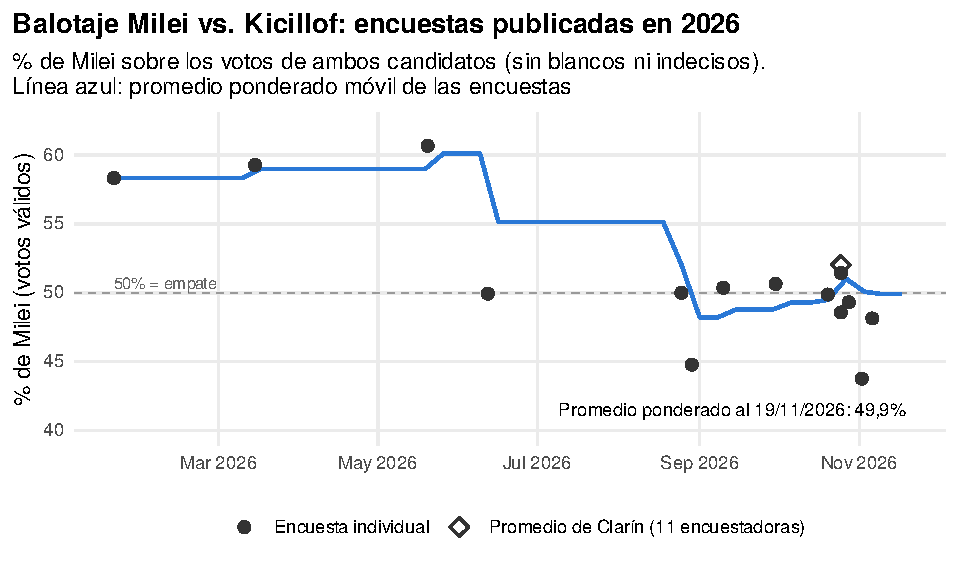
\includegraphics[width=0.85\textwidth]{fig_encuestas_balotaje.pdf}
  \caption{Encuestas de balotaje publicadas en 2026 y promedio ponderado móvil.
  Por encima de la línea punteada gana Milei; por debajo, Kicillof.}
  \label{fig:tracker}
\end{figure}

En primera vuelta (tabla~\ref{tab:pv1} y figura~\ref{fig:pv}) LLA queda
primera en los tres escenarios. Con el PRO aliado (A) llega a \pvLLA\% de los
votos afirmativos contra \pvPJ\% del peronismo, por encima del 45\% que alcanza
para ganar sin balotaje. Con el PRO por separado (B) baja a \pvSinproLLA\% y la
diferencia queda por debajo de los 10 puntos, por lo que habría balotaje. Con
las encuestas por candidato (C) hay prácticamente un empate: \pvCandLLA\%
contra \pvCandPJ\%.

\begin{table}[htbp]
\centering
\caption{Primera vuelta proyectada (\% de votos afirmativos). Entre corchetes,
el intervalo del 90\% simulado a octubre de 2027.}
\label{tab:pv1}
\small
\begin{tabular}{lccc}
\toprule
Fuerza & A. PRO aliado & B. PRO separado & C. Por candidato \\
\midrule
\tablainput{../results/tabla_primera_vuelta.tex}
\bottomrule
\end{tabular}
\end{table}

\begin{figure}[htbp]
  \centering
  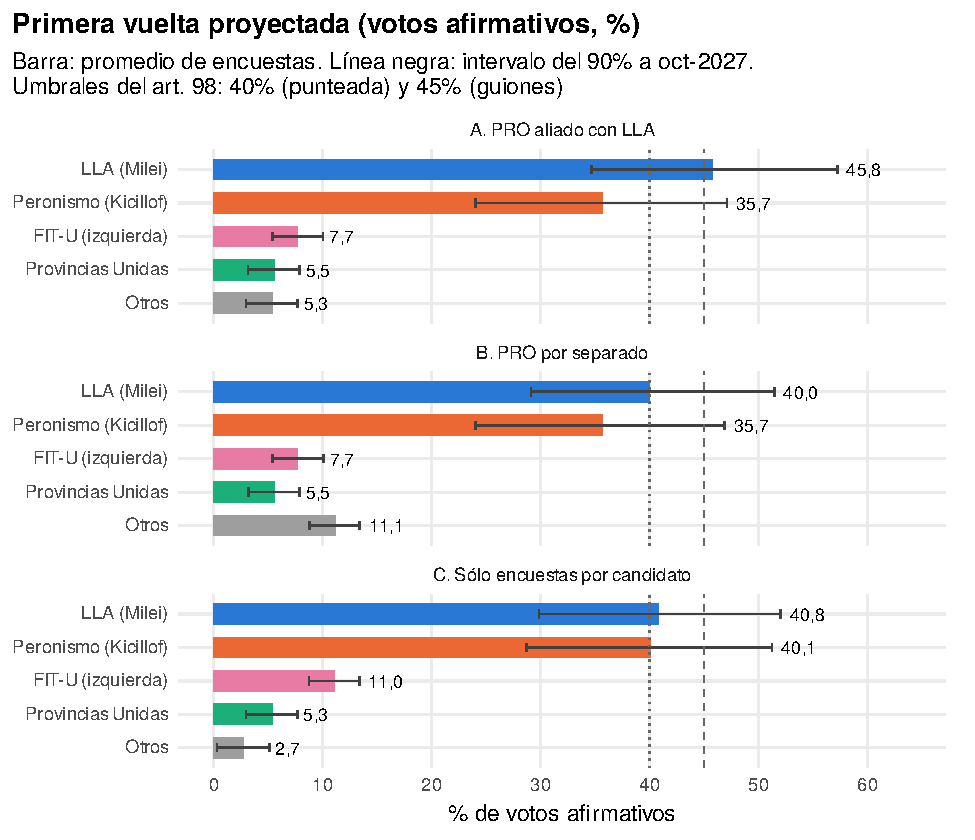
\includegraphics[width=0.8\textwidth]{fig_primera_vuelta.pdf}
  \caption{Primera vuelta proyectada por escenario, con su intervalo del 90\%
  y los umbrales constitucionales de 40\% y 45\%.}
  \label{fig:pv}
\end{figure}

\subsection{¿Quién gana la presidencia?}

La tabla~\ref{tab:pres} y la figura~\ref{fig:prob} resumen las \nSim{}
simulaciones de cada escenario.

\begin{table}[htbp]
\centering
\caption{Probabilidad de cada resultado presidencial (\% de las simulaciones).
La columna \textbf{Final} promedia los escenarios A y B.}
\label{tab:pres}
\small
\begin{tabular}{lccccc}
\toprule
Resultado & Hoy (A) & A. PRO aliado & B. PRO separado & C. Por candidato & \textbf{Final} \\
\midrule
\tablainput{../results/tabla_presidencial.tex}
\bottomrule
\end{tabular}
\end{table}

\begin{figure}[htbp]
  \centering
  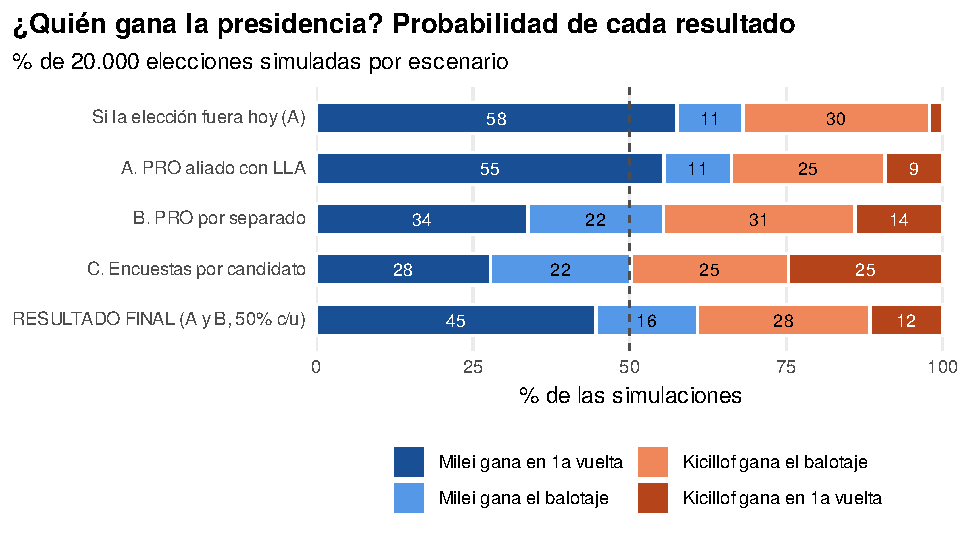
\includegraphics[width=0.9\textwidth]{fig_probabilidades.pdf}
  \caption{Probabilidad de cada resultado por escenario. Los tonos oscuros son
  triunfos en primera vuelta y los claros, en balotaje.}
  \label{fig:prob}
\end{figure}

\textbf{Resultado final.} Milei es reelecto en el \textbf{\pMileiFinal\%} de las
simulaciones: en el \pMileiPVFinal\% gana en primera vuelta y en el
\pMileiBalFinal\% gana el balotaje. Kicillof gana en el \textbf{\pKiciFinal\%}:
\pKiciPVFinal\% en primera vuelta y \pKiciBalFinal\% en el balotaje. La votación
mediana proyectada en primera vuelta es \votoLLAFinal\% para LLA (intervalo del
90\%: \votoLLAFinalLo--\votoLLAFinalHi) y \votoPJFinal\% para el peronismo
(\votoPJFinalLo--\votoPJFinalHi). Los intervalos son anchos porque faltan once
meses y porque las encuestas argentinas tienen errores grandes.

\textbf{¿Hay balotaje y quién lo gana?} Hay balotaje en el \pBalFinal\% de las
simulaciones. Aunque las encuestas de balotaje dan un empate, cuando el balotaje
efectivamente ocurre Milei lo gana sólo en el \pMileiCondFinal\% de los casos.
La razón está en la figura~\ref{fig:balotaje}: el balotaje ocurre sobre todo en
las simulaciones en las que a Milei le va peor de lo esperado en primera vuelta
(si le va como dicen las encuestas en el escenario A, gana directamente), y como
el error de las dos vueltas está correlacionado, en esas simulaciones también le
va peor en el balotaje. La mediana de Milei en el balotaje pasa de \balMedTodas\%
considerando todas las simulaciones a \balMedCond\% considerando sólo aquellas
en las que hay balotaje.

\begin{figure}[htbp]
  \centering
  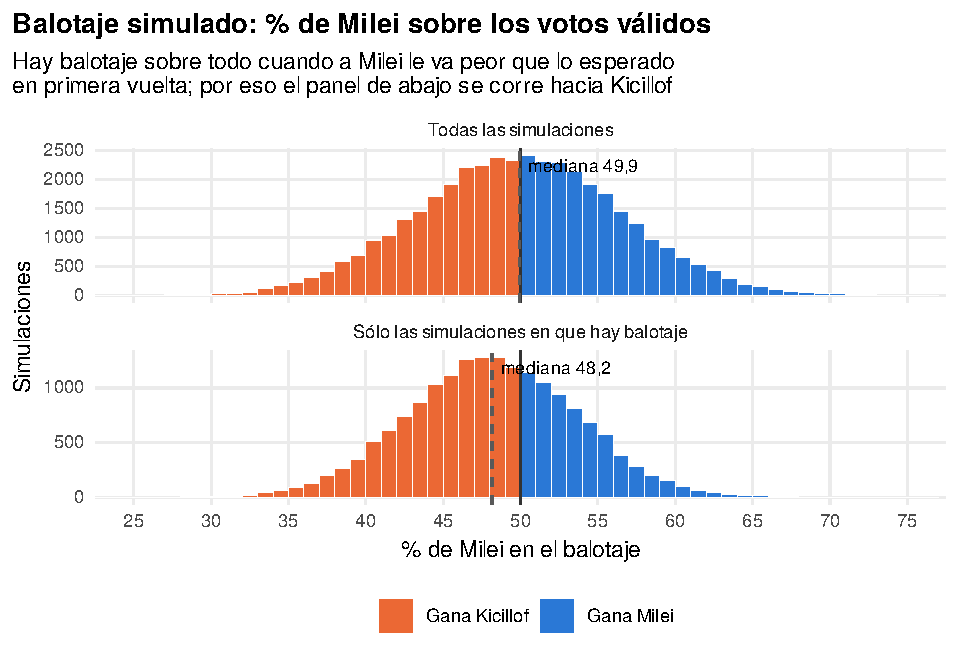
\includegraphics[width=0.8\textwidth]{fig_balotaje.pdf}
  \caption{Proporción de Milei en el balotaje simulado (escenarios A y B). Arriba,
  todas las simulaciones; abajo, sólo aquellas en las que efectivamente hay
  balotaje.}
  \label{fig:balotaje}
\end{figure}

\subsection{Sensibilidad: ¿de qué depende el resultado?}

\textbf{Alianza LLA--PRO.} Es el supuesto que más mueve el resultado: con el PRO
aliado, Milei gana en el \pMileiA\% de las simulaciones; con el PRO por separado,
en el \pMileiB\%. La diferencia viene casi toda de la primera vuelta (\pMileiPVA\%
contra \pMileiPVB\% de triunfos sin balotaje).

\textbf{Qué encuestas se miran.} Las encuestas por espacio (el promedio de
Clarín) muestran a LLA bastante arriba del peronismo, pero las que preguntan por
candidatos muestran un empate. Usando sólo estas últimas (escenario C) la
elección queda pareja: \pMileiC\% contra \pKiciC\%. Una explicación posible, que
señala el promedio de La Capital de Mar del Plata, es que muchas encuestas miden
al peronismo kirchnerista separado del no kirchnerista \cite{lacapital2026}.

\textbf{Cambio hasta la elección.} La tabla~\ref{tab:deriva} muestra que el
supuesto sobre cuánto puede cambiar la opinión en once meses importa menos: la
probabilidad de Milei va de \pMileiDerivaCero\% (sin cambio) a
\pMileiDerivaSiete\% (desvío de 7 puntos). A más incertidumbre, más cerca del
50\%.

\begin{table}[htbp]
\centering
\caption{Sensibilidad al desvío supuesto del cambio de opinión hasta octubre de
2027 (escenario A).}
\label{tab:deriva}
\small
\begin{tabular}{ccc}
\toprule
Desvío de la deriva (pp) & Milei gana (\%) & Hay balotaje (\%) \\
\midrule
\tablainput{../results/tabla_deriva.tex}
\bottomrule
\end{tabular}
\end{table}

\begin{figure}[htbp]
  \centering
  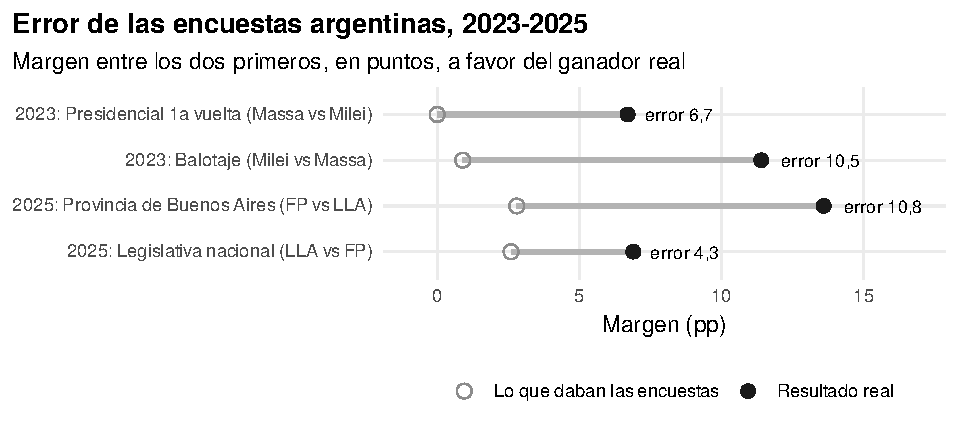
\includegraphics[width=0.8\textwidth]{fig_errores.pdf}
  \caption{Margen entre los dos primeros que daban las encuestas y margen real en
  cuatro elecciones recientes. En las cuatro las encuestas subestimaron al
  ganador.}
  \label{fig:errores}
\end{figure}

\begin{table}[htbp]
\centering
\caption{Error histórico de las encuestas argentinas (margen entre los dos
primeros, en puntos).}
\label{tab:errores}
\footnotesize
\begin{tabular}{p{5.6cm}crrrc}
\toprule
Elección & Fecha & Encuestas & Real & Error & Fuente \\
\midrule
\tablainput{../results/tabla_errores.tex}
\bottomrule
\end{tabular}
\end{table}

\FloatBarrier
\subsection{Gobernaciones}

\textbf{Efecto oficialismo.} En cinco de las siete elecciones provinciales de
2025 la fuerza del gobernador sacó bastante más que en la legislativa nacional
(figura~\ref{fig:efecto}). La ventaja fue mayor cuando se elegía gobernador
(\muDeltaGob\pp{} en promedio en Corrientes y Santiago del Estero) que en las
legislativas provinciales (\muDeltaLeg\pp). En Chaco y Misiones fue
prácticamente nula.

\begin{figure}[htbp]
  \centering
  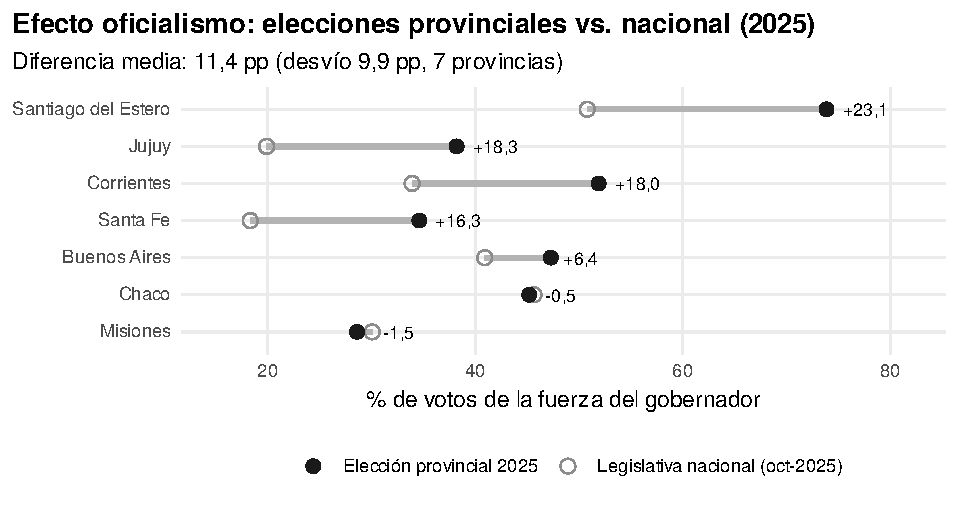
\includegraphics[width=0.85\textwidth]{fig_efecto_oficialismo.pdf}
  \caption{La fuerza del gobernador en la elección provincial de 2025 y en la
  legislativa nacional de octubre de 2025. El número es la diferencia en puntos.}
  \label{fig:efecto}
\end{figure}

\begin{table}[htbp]
\centering
\caption{Calibración del efecto oficialismo con las elecciones provinciales de
2025 (\% de la fuerza del gobernador).}
\label{tab:efecto}
\footnotesize
\begin{tabular}{llrrrc}
\toprule
Provincia & Tipo de elección & Provincial & Nacional & $\delta$ & Fuente \\
\midrule
\tablainput{../results/tabla_efecto.tex}
\bottomrule
\end{tabular}
\end{table}

\begin{table}[htbp]
\centering
\caption{Encuestas provinciales usadas.}
\label{tab:encprov}
\footnotesize
\begin{tabular}{llcL{5.5cm}cc}
\toprule
Distrito & Encuestadora & Fecha & Detalle & Ofic. / retador & Fuente \\
\midrule
\tablainput{../results/tabla_encuestas_prov.tex}
\bottomrule
\end{tabular}
\end{table}

\textbf{Resultado final por distrito.} La tabla~\ref{tab:gob} y las
figuras~\ref{fig:gob} y~\ref{fig:mapa} muestran el resultado final. El
oficialismo es el favorito en los \nOfiFavorito{} distritos, en línea con lo que
ocurrió en las elecciones provinciales de 2025. Pero ser favorito no es ganar
seguro: sumando las probabilidades, se esperan en promedio \cambiosEsperados{}
gobernaciones que cambian de manos, y la probabilidad de que todos los
oficialismos retengan es de apenas \pTodosRetienen\% (escenario base). Los
distritos más disputados son Santa Cruz (\pSantaCruz\%), Jujuy (\pJujuy\%) y Río
Negro (\pRioNegro\%), donde LLA (o, en Santa Cruz, el peronismo) queda cerca. En
la provincia de Buenos Aires el oficialismo peronista retiene en el \pPBA\% de
las simulaciones, con una votación mediana de \medPBAofi\% contra \medPBAseg\% de
LLA.

Las alianzas cambian mucho algunos resultados. En Santa Fe, si Provincias Unidas
y LLA compiten por separado, el oficialismo retiene en el \pSantaFeBase\% de los
casos y LLA queda prácticamente empatada; si se alían, en el \pSantaFeAlt\%. En la
Ciudad de Buenos Aires, con LLA y PRO juntos el oficialismo retiene en el
\pCabaBase\%, y por separado el PRO gana en el \pCabaAlt\% (con LLA y el
peronismo como competidores).

\begin{table}[htbp]
\centering
\caption{Resultado final de las 22 gobernaciones: probabilidad (\%) de que gane
el oficialismo y la de su principal retador. La última columna muestra la
probabilidad del oficialismo en el escenario base y en el alternativo (con
alianza con LLA, o PRO y LLA separados en CABA); el resultado final es el
promedio. Candidato: el que figura en las fuentes (``a definir'' si no hay uno).}
\label{tab:gob}
\scriptsize
\setlength{\tabcolsep}{3.5pt}
\begin{tabular}{L{2.3cm}L{4.1cm}L{2.2cm}cL{3.1cm}cc}
\toprule
Distrito & Fuerza oficialista & Candidato & P(ofic.) & Principal retador & P(ret.) & Base / alt. \\
\midrule
\tablainput{../results/tabla_gobernaciones.tex}
\bottomrule
\end{tabular}
\end{table}

\begin{figure}[htbp]
  \centering
  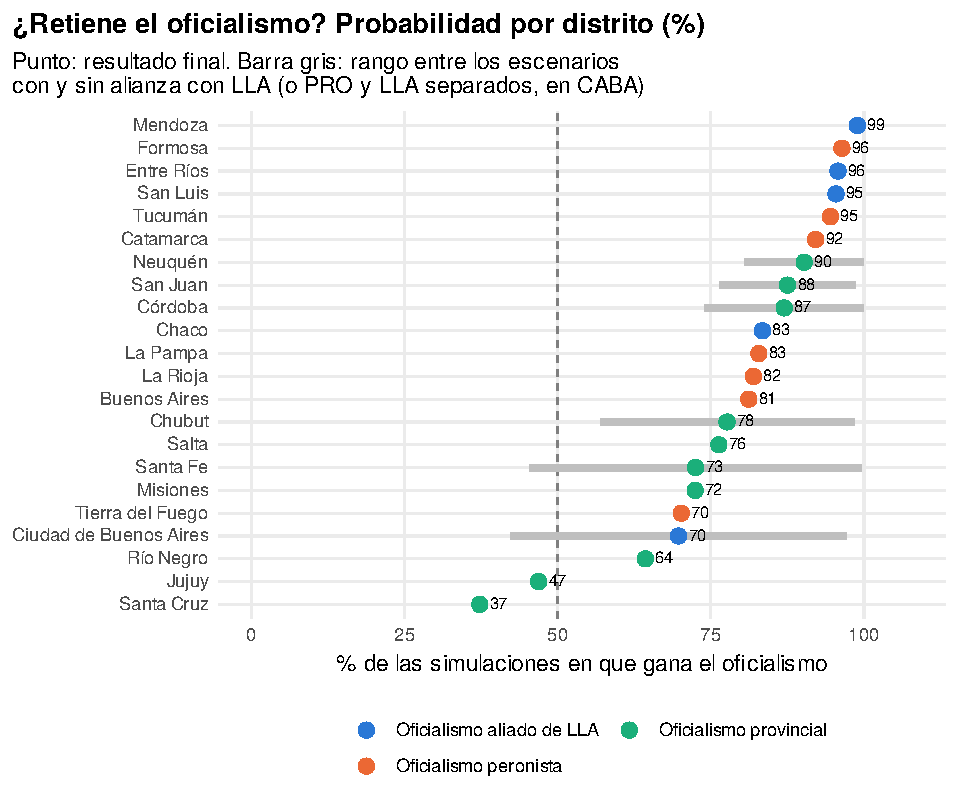
\includegraphics[width=0.8\textwidth]{fig_gobernaciones.pdf}
  \caption{Probabilidad de que el oficialismo retenga cada gobernación. La barra
  gris muestra el rango entre los escenarios con y sin alianza.}
  \label{fig:gob}
\end{figure}

\begin{figure}[htbp]
  \centering
  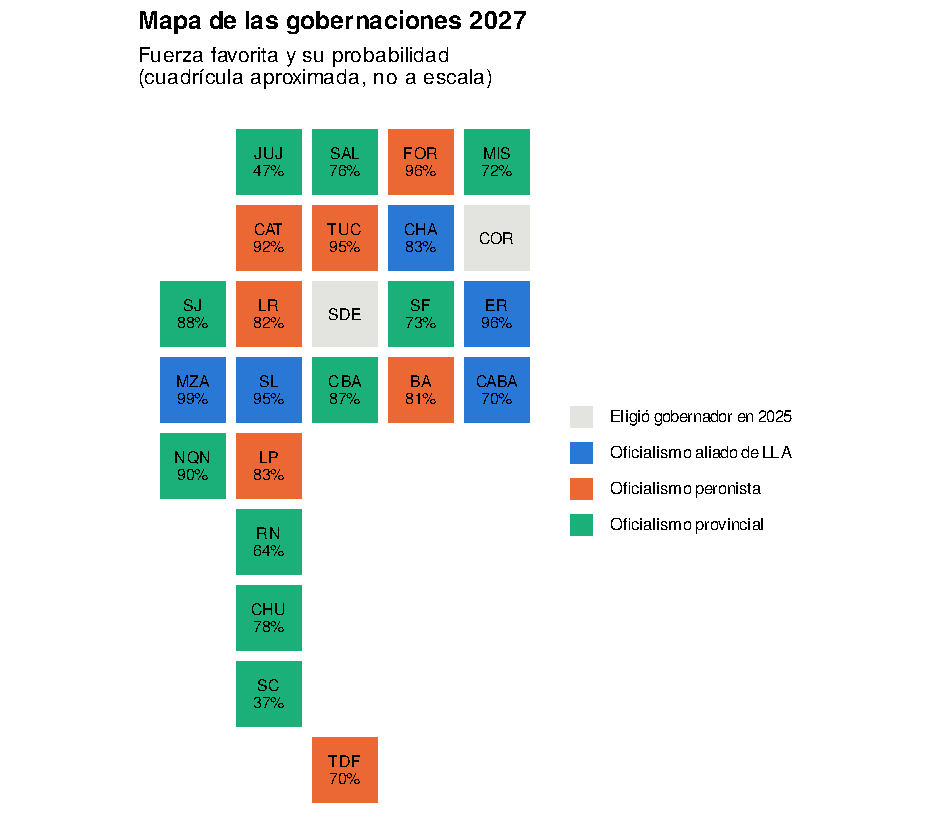
\includegraphics[width=0.72\textwidth]{fig_mapa.pdf}
  \caption{Mapa en cuadrícula de las gobernaciones 2027: tipo de oficialismo
  favorito y su probabilidad. Corrientes y Santiago del Estero eligieron
  gobernador en 2025.}
  \label{fig:mapa}
\end{figure}

\textbf{Votos proyectados.} La tabla~\ref{tab:votos} muestra la votación mediana
del oficialismo y de la segunda fuerza en cada distrito (escenario base).

\begin{table}[htbp]
\centering
\caption{Votación mediana proyectada (\% de votos válidos, escenario base).}
\label{tab:votos}
\footnotesize
\begin{tabular}{lrlr}
\toprule
Distrito & Oficialismo & Segunda fuerza & \% \\
\midrule
\tablainput{../results/tabla_votos_provinciales.tex}
\bottomrule
\end{tabular}
\end{table}

\textbf{Cuántas gobernaciones gana cada espacio.} La figura~\ref{fig:conteo}
muestra la distribución. En la mediana, LLA (sola o como parte de una alianza con
el oficialismo provincial) gana \gobLLAMed{} gobernaciones (intervalo del 90\%:
\gobLLALo--\gobLLAHi), el peronismo \gobPJMed{} (\gobPJLo--\gobPJHi) y los
partidos provinciales sin alianza con LLA \gobPROVMed{} (\gobPROVLo--\gobPROVHi).
El número de LLA incluye a los cinco oficialismos que ya compitieron aliados con
LLA en 2025.

\begin{figure}[htbp]
  \centering
  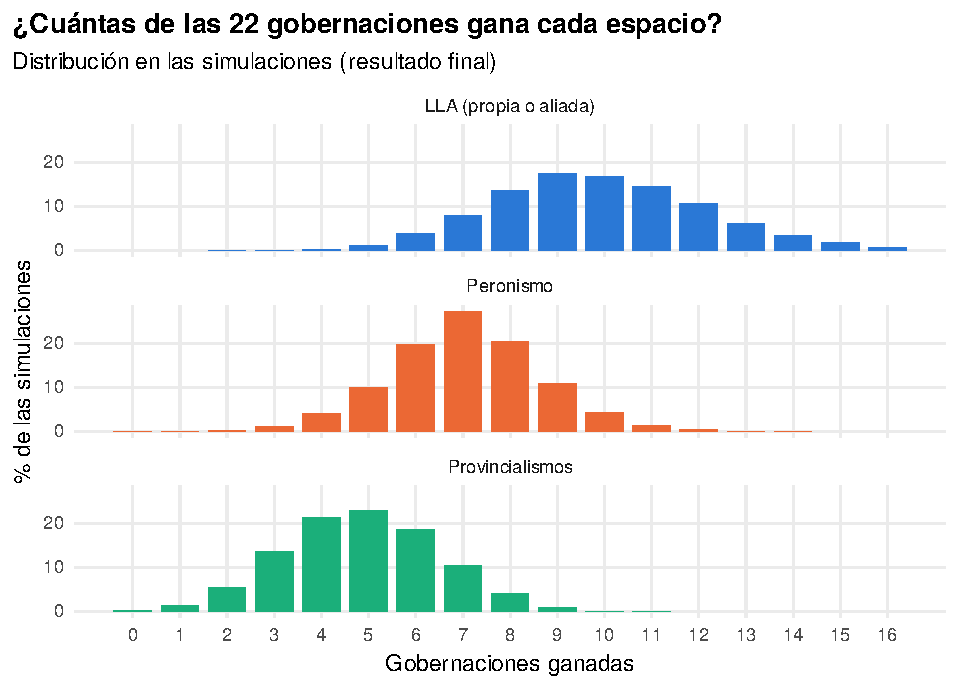
\includegraphics[width=0.75\textwidth]{fig_conteo_gobernaciones.pdf}
  \caption{Cantidad de gobernaciones ganadas por cada espacio en las simulaciones
  (resultado final).}
  \label{fig:conteo}
\end{figure}

\FloatBarrier
\subsection{Resultado final de la simulación}

\begin{center}
\fcolorbox{black!40}{black!4}{\parbox{0.92\textwidth}{\small
\textbf{Presidencia 2027--2031} (\nSim{} elecciones simuladas por escenario;
resultado final = promedio de los escenarios con y sin alianza LLA--PRO)
\begin{itemize}
  \item \textbf{Javier Milei (LLA): \pMileiFinal\%} de probabilidad de ser
        reelecto (\pMileiPVFinal\% en primera vuelta, \pMileiBalFinal\% en
        balotaje).
  \item \textbf{Axel Kicillof (Fuerza Patria): \pKiciFinal\%}
        (\pKiciPVFinal\% en primera vuelta, \pKiciBalFinal\% en balotaje).
  \item Primera vuelta proyectada: LLA \votoLLAFinal\%, peronismo
        \votoPJFinal\% (votos afirmativos, mediana).
  \item \textbf{Balotaje: \pBalFinal\%} de probabilidad. Si lo hay, Kicillof es
        favorito: Milei lo gana en el \pMileiCondFinal\% de los casos (mediana
        de Milei: \balMedCond\%; de Kicillof: \balMedCondK\%).
\end{itemize}
\textbf{Gobernaciones}: el oficialismo es favorito en los \nOfiFavorito{}
distritos (tabla~\ref{tab:gob}); se esperan \cambiosEsperados{} cambios de signo
en promedio. Los más abiertos: Santa Cruz, Jujuy y Río Negro. Mediana de
gobernaciones: LLA y aliados \gobLLAMed, peronismo \gobPJMed, provinciales
\gobPROVMed.

\medskip
\emph{Es una simulación probabilística con los datos disponibles al
\fechaCorte, no una predicción: con el escenario de encuestas por candidato la
elección presidencial es un empate (\pMileiC\% a \pKiciC\%).}
}}
\end{center}

% =====================================================================
\section{Conclusiones}

Con todos los datos públicos que pudieron reunirse, la simulación da a Javier
Milei como favorito para 2027 (\pMileiFinal\%), pero lejos de ser un resultado
seguro: en cuatro de cada diez simulaciones gana Axel Kicillof. El dato más
interesante es que el promedio de las encuestas de balotaje es un empate y, sin
embargo, el resultado global favorece a Milei. Eso pasa porque Milei tiene una
ventaja que las encuestas de balotaje no capturan: puede ganar en primera vuelta.
A la vez, si no logra ganar en primera vuelta, es porque las cosas le fueron peor
de lo que decían las encuestas, y entonces llega debilitado al balotaje. En las
provincias el patrón de 2025 se repite: los oficialismos son favoritos en todos
los distritos, aunque con varios casos abiertos.

\textbf{Ventajas del enfoque.}
\begin{itemize}
  \item Todos los datos son reales, públicos y tienen su fuente; cualquiera puede
        revisarlos y actualizarlos.
  \item Las incertidumbres clave (error de las encuestas y ventaja del
        oficialismo) se calibran con elecciones argentinas recientes y no se
        suponen.
  \item Se aplican las reglas constitucionales exactas y se tiene en cuenta la
        correlación entre las dos vueltas y entre las provincias.
  \item El resultado se presenta como probabilidades, con escenarios y
        sensibilidad, y el código es reproducible (semilla fija).
\end{itemize}

\textbf{Limitaciones.}
\begin{itemize}
  \item \textbf{Pocas encuestas y lejanas a la elección.} Hay \nEncBal{}
        encuestas de balotaje, tres de primera vuelta y \nEncProv{} provinciales,
        y faltan once meses. La literatura muestra que a esta distancia las
        encuestas predicen poco \cite{erikson2012,jennings2020}.
  \item \textbf{Candidatos no definidos.} Kicillof no es candidato oficial; si
        el peronismo elige a otra persona, o si cambian las alianzas, el
        resultado puede cambiar mucho. Lo mismo vale para las provincias donde
        el candidato figura ``a definir''.
  \item \textbf{Calibraciones con pocos casos.} El error de las encuestas se
        estima con cuatro elecciones y el efecto oficialismo con siete, de las
        cuales sólo dos fueron elecciones de gobernador (donde el efecto fue
        mayor). El cambio de opinión hasta la elección es un supuesto; en 2026 el
        promedio ya se movió unos diez puntos en seis meses.
  \item \textbf{Simplificaciones del modelo provincial.} El efecto oficialismo
        se resta proporcionalmente a las demás fuerzas, se usan sólo tres
        fuerzas por distrito y gana la más votada. No se modelan las reglas
        particulares de cada provincia (por ejemplo, el balotaje en la Ciudad de
        Buenos Aires y en Tierra del Fuego) ni las disputas judiciales sobre
        reelecciones (Tucumán, Salta, Formosa).
  \item \textbf{Encuestas por espacio y por candidato.} Ambas miden cosas
        distintas y dan resultados distintos; la decisión de cuál usar cambia el
        resultado presidencial (escenarios A, B y C).
\end{itemize}

\textbf{Trabajo futuro.}
\begin{itemize}
  \item Actualizar los datos a medida que salgan nuevas encuestas y se definan
        candidaturas y alianzas (el código está preparado para eso).
  \item Reemplazar el promedio ponderado por un modelo bayesiano dinámico con
        efecto casa de cada encuestadora \cite{linzer2013,heidemanns2020}.
  \item Agregar variables estructurales (economía, aprobación del gobierno) y
        modelar las reglas electorales de cada provincia.
  \item Simular también la composición del Congreso.
\end{itemize}

% =====================================================================
\section*{Reproducibilidad}
El proyecto completo (datos con fuentes, código R comentado con pre y
postcondiciones, figuras y este informe) se ejecuta abriendo
\texttt{Elecciones2027.Rproj} en RStudio y corriendo \texttt{main.R}; tarda menos
de un minuto. Sólo usa R base \cite{rcore} y \texttt{ggplot2}
\cite{wickham2016}. La semilla aleatoria está fija, así que los resultados son
idénticos en cualquier computadora.

\bibliographystyle{unsrtnat}
\bibliography{references}

% =====================================================================
\appendix
\section{Candidatos y situación de cada gobernación}

\begingroup
\scriptsize
\setlength{\tabcolsep}{3pt}
\begin{longtable}{L{1.7cm}L{2.1cm}L{2.0cm}L{3.3cm}L{2.3cm}L{2.6cm}c}
\caption{Situación de cada distrito para 2027, según las fuentes citadas.
``(oficialismo)'': esa fuerza es la que gobierna; ``(alianza con oficialismo)'':
LLA compite junto al gobernador.}
\label{tab:candidatos}\\
\toprule
Distrito & Gobernador & ¿Reelección? & Candidato del oficialismo & Candidato LLA & Peronismo / otros & Fuente \\
\midrule
\endfirsthead
\toprule
Distrito & Gobernador & ¿Reelección? & Candidato del oficialismo & Candidato LLA & Peronismo / otros & Fuente \\
\midrule
\endhead
\bottomrule
\endfoot
\tablainput{../results/tabla_candidatos.tex}
\end{longtable}
\endgroup

\end{document}
